\chapter{Multi User Interaktion}
\label{ch:Multi_User_Interaktion}

\section{Realisierung}
Mit dem Projekt und den Erkenntnissen des Single-User Prototypen begann die Erstellung eines Multi-User tauglichen Prototypen.

\subsection{Multi User}
\label{ch:multi_user}
Um die Applikation Multi-User tauglich zu machen, wurde die Photon-Engine verwendet (\cite{noauthor_photon_2019}). Entwickelt wurde diese von der Firma Exit Games. Diese Firma stellt ein Unity-Asset zur Verfügung mit verschiedenen Beispielen wie das Asset zusammen mit der Photon-Engine einzusetzen ist. \\

\noindent Auf der Webseite von Photon kann nach einem erfolgreichen Login eine neue Applikation erstellt werden. Für den Multi-User Prototyp wurde eine Realtime-Applikation erstellt mit bis zu 20 gleichzeitigen Benutzern. Soll eine Applikation mit mehr als 20 gleichzeitigen Nutzern erstellt werden, wird dies kostenpflichtig. Nach dem erstellen kann die erhaltene App ID, zu sehen in Abbildung \ref{fig:photon_dashboard}, in Unity verwendet werden.

\begin{figure}[h!]
	\centering
	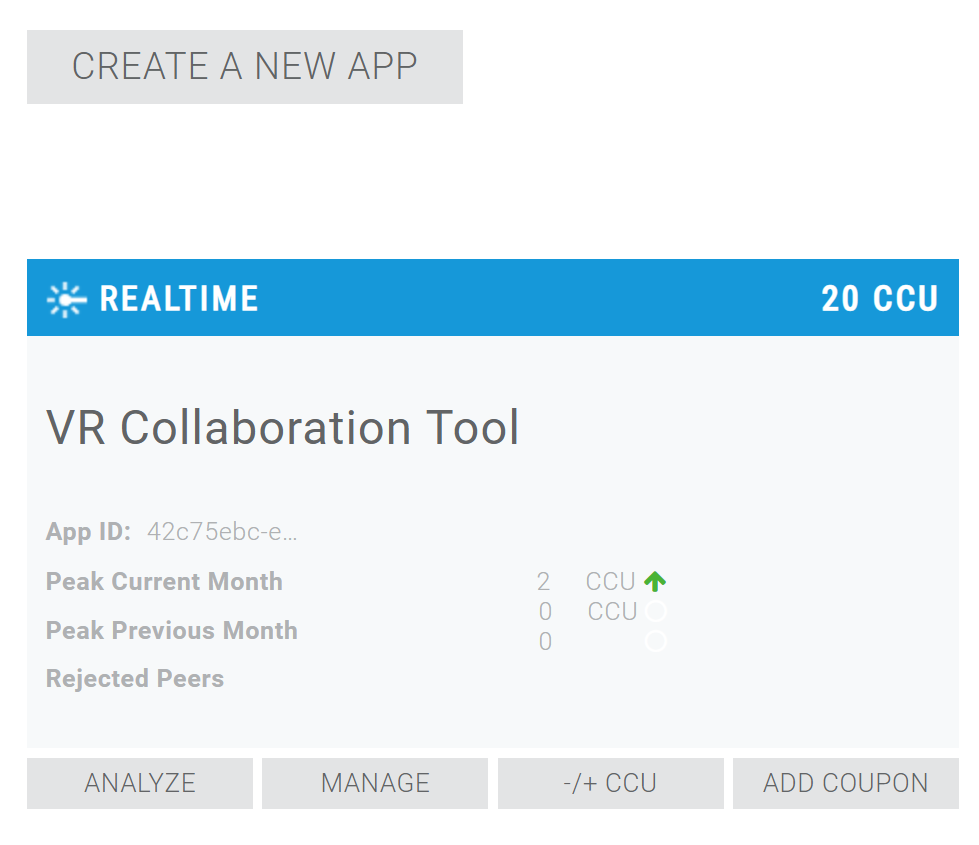
\includegraphics[keepaspectratio,width=0.4\linewidth]{img/Photon_Dashboard.PNG}
	\caption{Photon Dashboard}
	\label{fig:photon_dashboard}
\end{figure} 

Mit der App ID kann Unity sich nun auf die Applikation verbinden. Die erste Instanz, welche sich verbindet wird automatisch als Master deklariert. Um nun mit anderen Instanzen kommunizieren zu können, müssen diese sich mit einen virtuellen Raum verbinden. Sobald sich beide im gleichen Raum befinden, kann die Kommunikation beginnen.\\
Jeglichen Objekten, welche nun untereinander synchronisiert werden sollen, muss die Komponente Photon View hinzugefügt werden. Diese besitzt die folgenden Parameter:
\begin{itemize} [itemsep=1pt]
	\item Owner: Der aktuelle Besitzer der Objekts
	\item View ID: Eindeutige Identität des Objektes
	\item Observed Components: Welche Komponenten des Objektes mit den anderen Instanzen synchronisiert werden soll.
\end{itemize}

Für die Synchronisation vieler standardmässigen Unity-Komponenten stellt die Photon-Engine schon Komponenten zur Verfügung. Eine dieser Komponenten, die Photon Transform View, wurde im Prototyp verwendet, um die Position und die Rotation des Objektes zu synchronisieren. Somit werden diese beiden Eigenschaften mit allen Instanzen synchronisiert, welche nicht Besitzer des Objektes sind. Es ist aber nicht möglich als Nicht-Besitzer ein Objekt zu bewegen. \\
Die Master-Instanz wird bei der Initialisierung Besitzer von allen Objekten, welche eine Photon View besitzen. Um als Nicht-Master-Instanz nun ein Objekt bewegen zu können, stellt die Photon-Engine die Funktion \textit{RequestOwnership()} zur Verfügung. Diese Funktion macht die Instanz zum neuen Besitzer der Photon View, welche die Funktion aufgerufen hat. Somit kann nun die Nicht-Master-Instanz das Bauteil bewegen und alle anderen Instanzen sehen diese Bewegung. \\

\noindent Da die Bauteile im Prototyp einen Rigidbody angehängt haben, muss auch dieser synchronisiert werden. Die Photon-Engine stellt aber für die Synchronisation eines Rigidbody keine Komponenten zur Verfügung. Sie stellt aber die Methode \textit{OnPhotonSerializeView(PhotonStream stream, PhotonMessageInfo info)} zur Verfügung, mit welcher eigene Attribute zwischen den Instanzen synchronisiert werden können. Die Methode wird standardmässig 10 mal in der Sekunde aufgerufen, kann aber in den Einstellungen angepasst werden. Nachfolgend ein Ausschnitt wie der Aufbau dieser Methode aussehen sollte.

\begin{algorithm}
	\KwIn{PhotonStream, PhotonMessageInfo}
	\eIf{Falls die aktuelle Instanz auf den Stream schreiben kann} {
		Schreibe alle Informationen des Rigidbody auf den Stream\;
		Schreibe weitere Attribute auf den Stream\;
	}{
		Lese die Informationen aus dem Stream und speichere diese in den Rigidbody\;
		Lese die weiteren Attribute aus dem Stream\;	
	}
\end{algorithm}

Eine Instanz kann nur dann auf den Stream schreiben, wenn sie in besitzt der Photon View ist. Die Komponente Photon Transform View funktioniert sehr ähnlich wie der beschriebene Pseudocode.

\subsection{Avatar-Repräsentation in der virtuellen Umgebung}

Wie in Kapitel \ref{ch:avatar_repraesentation_realisierung} beschrieben, wurde für diesen Prototyp ein einfacher Avatar bestehend aus Kopf, Oberkörper und den beiden Händen umgesetzt. Dieser ist in Abbildung \ref{fig:avatar} zu sehen mit Controllern als Hände. Die Position und Rotation des Oberkörpers werden anhand der Position sowie der Rotation des Kopfes berechnet.

\begin{figure}[h!]
	\centering
	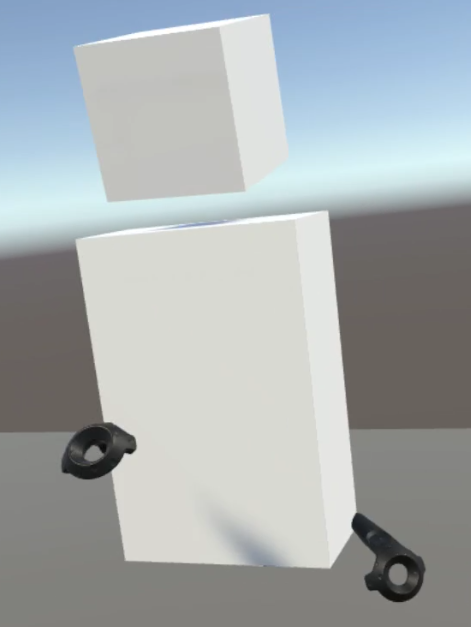
\includegraphics[keepaspectratio,width=0.4\linewidth]{img/Avatar.PNG}
	\caption{Avatar leicht nach links blickend}
	\label{fig:avatar}
\end{figure} 

Der Benutzer selbst sieht von seinem eigenen Avatar nur die Hände mit den Controllern. Der Oberkörper sowie der Kopf sind für ihn unsichtbar, da sie sonst in der Quere des Sichtfelds sein würden. Um den Avatar mit den anderen Instanzen zu synchronisieren wurde ebenfalls, wie in Kapitel \ref{ch:multi_user} beschrieben, auf jede Komponente des Avatars eine Photon View hinzugefügt. Somit sehen die Benutzer sich untereinander und können mithilfe von Gesten miteinander Kommunizieren.

\subsection{Kommunikation zwischen den Benutzern}
\label{ch:kommunikation_zwischen_benutzern_realisierung}
Für die Kommunikation zwischen den Benutzern wurde ebenfalls auf die Photon-Engine zurückgegriffen. Im Photon Dashboard, zu sehen in Abbildung \ref{fig:photon_dashboard}, wurde eine Voice Applikation erstellt und die erhaltene App ID konnte dann in Unity, zusätzlich zu der App ID für die Realtime-Applikation, eingeben werden. \\

\noindent Um die Voice Applikation nutzen zu können, muss einem leeren GameObject in der Szene eine \grqq Photon Voice Network\grqq{} Komponente sowie ein \grqq Recorder\grqq{} hinzugefügt werden. Diese Komponenten sind ebenfalls aus einem Plugin der Photon-Engine namens Photon Voice (\cite{noauthor_photon_2019-1}). So wird der Sound über das Mikrophon des Benutzers aufgenommen. Für die Wiedergabe wurde dem Avatar zusätzlich eine \grqq Speaker\grqq{}-Komponente, welche ebenfalls aus dem Photon Voice Plugin stammt, hinzugefügt. Somit können die Benutzer miteinander über grosse Distanzen kommunizieren. 

\subsection{Gleichzeitige Interaktion am selben Objekt}
\label{ch:gleichzeitige_interaktion_realisierung}

Durch die Erkenntnisse während Arbeit mit der Photon-Engine wurde klar, dass eine simultane Interaktion am selben Objekt nicht möglich ist, da immer nur ein Benutzer Besitzer eines Bauteils sein kann. Da nur der Besitzer das Bauteil verschieben kann, müssten andere Technologien verwendet werden. Im Kapitel \ref{ch:gleichzeitige_interaktion} wurde entschieden, die beiden Varianten «First come, First grab» und Zauberstab zu implementieren. Beide Varianten verlangen keine simultane Interaktion am selben Objekt und konnten daher umgesetzt werden. \\

\noindent Die Variante «First come, First grab» funktioniert wie folgt. Alle Benutzer können Bauteile greifen und diese verschieben solange kein anderer das Bauteil aktuell am manipulieren ist. Der genaue Ablauf ist im nachfolgenden Pseudocode veranschaulicht.

\begin{algorithm}
	Der Benutzer versucht das Bauteil zu greifen\;
	\eIf{Ist das Bauteil noch greifbar?} {
		\textit{RequestOwnerShip()} aufrufen um Besitzer des Bauteils zu werden\;
		Das Bauteil für anderen Benutzer sperren\;
		Das Bauteil an die Hand des Benutzers anhängen\;
		
	}{
		Dem Benutzer mitteilen, dass das Bauteil aktuell nicht greifbar ist\;	
	}
\end{algorithm}

Für die zweite Variante würde dem Prototypen ein Zauberstab hinzugefügt, welcher ebenfalls greifbar und mit einer Photon View sowie einer Photon Transform View ausgestattet ist. Somit wird die Position wie auch die Rotation zwischen allen Benutzern synchronisiert. Nur derjenige Benutzer, welcher aktuell in Besitz des Zauberstabs ist, kann Bauteile manipulieren. Um den Zauberstab nicht immer in der Hand halten zu müssen, wird dieser beim greifen rechts bzw. links neben der Hand platziert und bewegt sich mit dieser mit, siehe Abbildung \ref{fig:magic_wand}. Möchte ein anderer Benutzer die virtuelle Umgebung manipulieren muss er den Zauberstab vom aktuellen Benutzer übernehmen, indem er den Zauberstab an der Hand des anderen Benutzers greift.

\begin{figure}[h!]
	\centering
	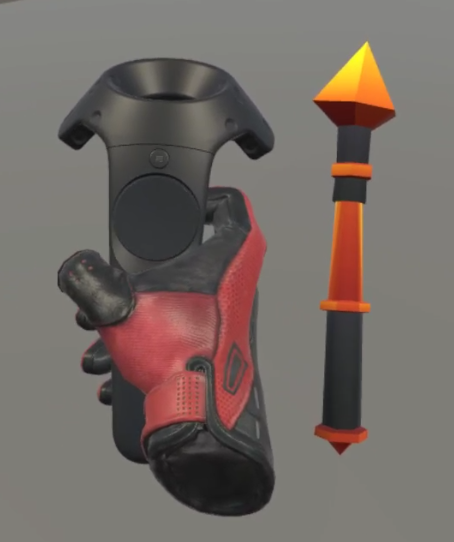
\includegraphics[keepaspectratio,width=0.25\linewidth]{img/MagicWand.PNG}
	\caption{Zauberstab angehängt an der rechten Hand}
	\label{fig:magic_wand}
\end{figure} 

\section{Evaluation}
Nach Fertigstellung des Multi-User Prototypen wurde ebenfalls, wie schon nach dem ersten Prototypen, eine Nutzerstudie durchgeführt. Anhand dieser Nutzerstudie sollte evaluiert werden, welche der beschriebenen Varianten im Kapitel \ref{ch:gleichzeitige_interaktion_realisierung} sich besser für die Anwendung eignet.

\subsection{Aufgabenstellung}
Für diesen Nutzertest wurden immer zwei Teilnehmer gleichzeitig benötigt. Falls einer von beiden noch keine Erfahrungen mit Virtual Reality hatte, oder sein Partner noch nicht Verfügbar war, wurde ihnen das Bogenschiessen im Spiel \grqq The Lab\grqq{} gezeigt (\cite{noauthor_lab_2019}). Hier ging es darum, dass sich die Teilnehmer vor dem Benutzen der Multi-User Applikation mit Virtual Reality vertraut machen konnten. \\

\noindent Anschliessend war es die Aufgabe zusammen vier verschiedene Motoren zusammenzubauen. Zweimal mit der Variante «First come, First grab» und zweimal mit der Variante mit dem Zauberstab. \\
Dafür hat immer einer der beiden Teilnehmer gesehen an welche Position das Bauteil muss (Abbildung \ref{fig:wohin}) und der andere hat gesehen, welches Bauteil an diese Stelle muss (Abbildung \ref{fig:welches}). Dies wechselte immer zwischen den Teilnehmer. So wurde die Zusammenarbeit forciert, dass nicht einer alles alleine machen konnte.

\begin{figure}[h!]
	\centering
	\begin{minipage}[b]{0.49\linewidth}
		\centering
		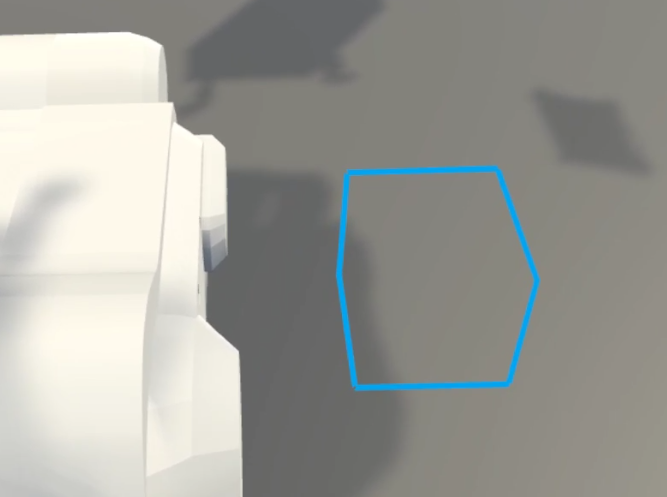
\includegraphics[keepaspectratio,width=0.9\linewidth]{img/Wohin.PNG}
		\caption{Wohin muss das Bauteil?}
		\label{fig:wohin}
	\end{minipage}
	\hfill
	\begin{minipage}[b]{0.49\linewidth}
		\centering
		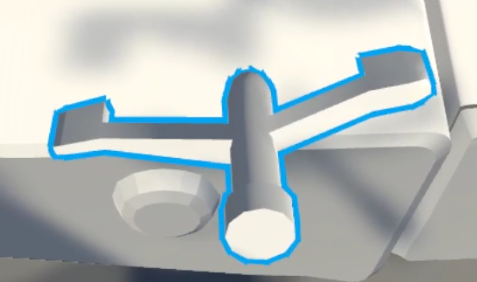
\includegraphics[keepaspectratio,width=0.9\linewidth]{img/Welches.PNG}
		\caption{Welches Bauteil ist es?}
		\label{fig:welches}
	\end{minipage}
\end{figure}

\subsection{Resultat}
An der zweiten Nutzerstudie haben 13 Nutzer teilgenommen. Alle Teilnehmer bekamen für die Teilnahme an der Nutzerstudie einen 10.- CHF Gutschein für Digitec Galaxus. Einige Teilnehmer hatten noch keine Erfahrungen mit Virtual Reality. \\

\noindent Den Teilnehmern wurden nach dem Abschluss der Aufgaben die folgenden vier Fragen gestellt:

\begin{enumerate} [itemsep=1pt,topsep=0pt]
	\item Frage: Wie gut funktionierte die Interaktion mit der anderen Person? \\
	Auswertung: Alle Teilnehmer fanden die Interaktion mit der anderen Person sehr angenehm und intuitiv. \grqq Anderer Avatar zu sehen ist sehr hilfreich\grqq{}, meinte ein Teilnehmer und viele andere schrieben, dass der Avatar ein sehr wichtiger Punkt für die Interaktion mit anderen war. Insbesondere, da die Teilnehmer untereinander mithilfe von Gesten kommunizieren konnten, zusätzlich zu der Stimme.  \\
	Eine Person bemängelte, dass der Avatar den anderen Bauteilen zu ähnlich sah, da beide eine weisse Farbe hatten.
	\item Frage: Sehen Sie einen Mehrwert in der Applikation gegenüber traditionellen Methoden über ein Bauteil / eine Maschine zu diskutieren? \\
	Auswertung: Alle Teilnehmer sahen einen Mehrwert in der Applikation gegenüber traditionellen Methoden. Viele fanden, dass es so einfacher sei sich etwas vorstellen zu können, da der Benutzer um das Objekt rumlaufen oder es gar bewegen kann. Ein Benutzer meinte, dass die Applikation für Schulungen bei heikleren Objekten verwendet werden könne: \grqq Für Schulungen bei heikleren Objekten\grqq{}\\
	\grqq Aber solange teure Hardware benötigt wird, eher unrealistisch\grqq{}, schrieb ein Teilnehmer, da für die meisten VR-Brillen heutzutage noch ein teurer Computer benötigt wird.

	\item Frage: Welche der beiden Varianten fanden Sie hilfreicher, um den Task auszuführen und wieso? \\
	Auswertung: \grqq Erste Variante war besser, da man besser zusammenarbeiten konnte\grqq{}, oder ähnliche Aussagen wurden von allen Teilnehmern gemacht. Es sei, bei dieser spezifischen Aufgabe besser gewesen, wenn beide Teilnehmer die gleichzeitig mit den Bauteilen interagieren konnten.\\
	Viele Teilnehmer können sich aber vorstellen, dass die Variante mit dem Zauberstab vor allem in Lernumgebungen oder Präsentation mit mehreren Personen hilfreich sein könnte. So interagieren nicht ungewollt Benutzer mit Objekten, falls dies nicht erwünscht ist. Die Aussage eines Teilnehmers fasst dies gut zusammen: \grqq Zweite Variante eher beim Vorzeigen, oder Fachpersonal bei welchem Input gegeben werden können. (zur Veranschaulichung)\grqq{} 
	
	\item Frage: Wenn Sie etwas an der Applikation ändern könnten, was wäre es? \\
	Auswertung: Viele Teilnehmer bemängelten den Zusammenbau, da der Teilnehmer mit dem blauen Würfel, zu sehen in Abbildung \ref{fig:wohin}, die Rotation des Bauteiles nicht sehen konnte. Dementsprechend kam es da zu grossen Verwirrungen wie das nächste Bauteil nun angemacht werden musste. Eine gute Rückmeldung bezüglich des Problems kam von einem Teilnehmer: \grqq Tisch auf welchem die Objekte zusammengebaut werden können. Das erste Teil sollte fix sein.\grqq{} \\
	Ein Teilnehmer fand, dass die Bauteile leicht verschiebbar sein sollten, ohne diese packen zu müssen: \grqq Teile sollten leicht stoss bar sein.\grqq{}
\end{enumerate}

\pagebreak
\subsection{Schlussfolgerung}
Die Teilnehmer der zweiten Nutzerevaluation waren mit dem Multi-User Prototyp sehr zufrieden. Leider kam es bei den gestellten Aufgaben öfters zu Problemen, da zum Beispiel richtig zusammengesetzte Bauteile als falsch zusammengebaut erkannt und der nächste Schritt nicht angezeigt wurde. Aber obwohl diese Probleme aufgetreten sind, haben die Teilnehmer die Maschine mithilfe von \grqq Trial and Error\grqq{} zusammenbauen können und hatten bemerkbar Freude dabei. \\

\noindent Anhand den Antworten der Teilnehmer haben beide Varianten Anwendungsgebiete. Die Variante \grqq First come, First grab\grqq{} kann für das gemeinsame arbeiten mit Objekten in der virtuellen Realität verwendet werden. Sobald es in den Bereich der Schulung geht oder ein Benutzer anderen was zeigen will, ohne dass diese mit den Objekten interagieren, würde sich die zweite Variante mit dem Zauberstab empfehlen.

\section{Systemarchitektur}
\begin{figure}[h!]
	\centering
	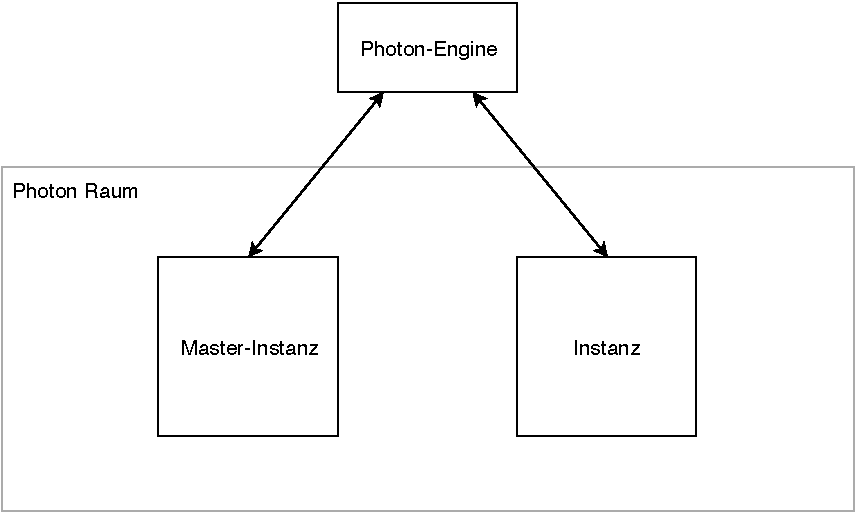
\includegraphics[keepaspectratio,width=0.60\linewidth]{img/ArchitekturT2.pdf}
	\caption{Systemarchitektur des Multi-User Prototypen}
	\label{fig:systemarchitektur_mutli_user}
\end{figure}

Die beiden Instanzen sind grundsätzlich genau gleich aufgebaut wie in der Single-User Applikation, beschrieben in Kapitel \ref{ch:systemarchitektur_single_user}. Um mit der Photon-Engine kommunizieren zu können musste zusätzlich noch das Photon-Engine Plugin sowie das Photon-Voice Plugin hinzugefügt werden. \\
Die erste Instanz, welche sich mit der Photon-Engine verbindet, wird automatisch zur Master-Instanz. Nach dem Verbinden mit der Photon-Engine wird die Instanz mit einem Photon-Raum verbunden. Sobald sich nun zwei Instanzen im selben Raum befinden, werden alle Objekte mit einer Photon View zwischen ihnen synchronisiert, beschrieben in Kapitel \ref{ch:multi_user}.

\section{Klassendiagramm}

\begin{figure}[h!]
	\centering
	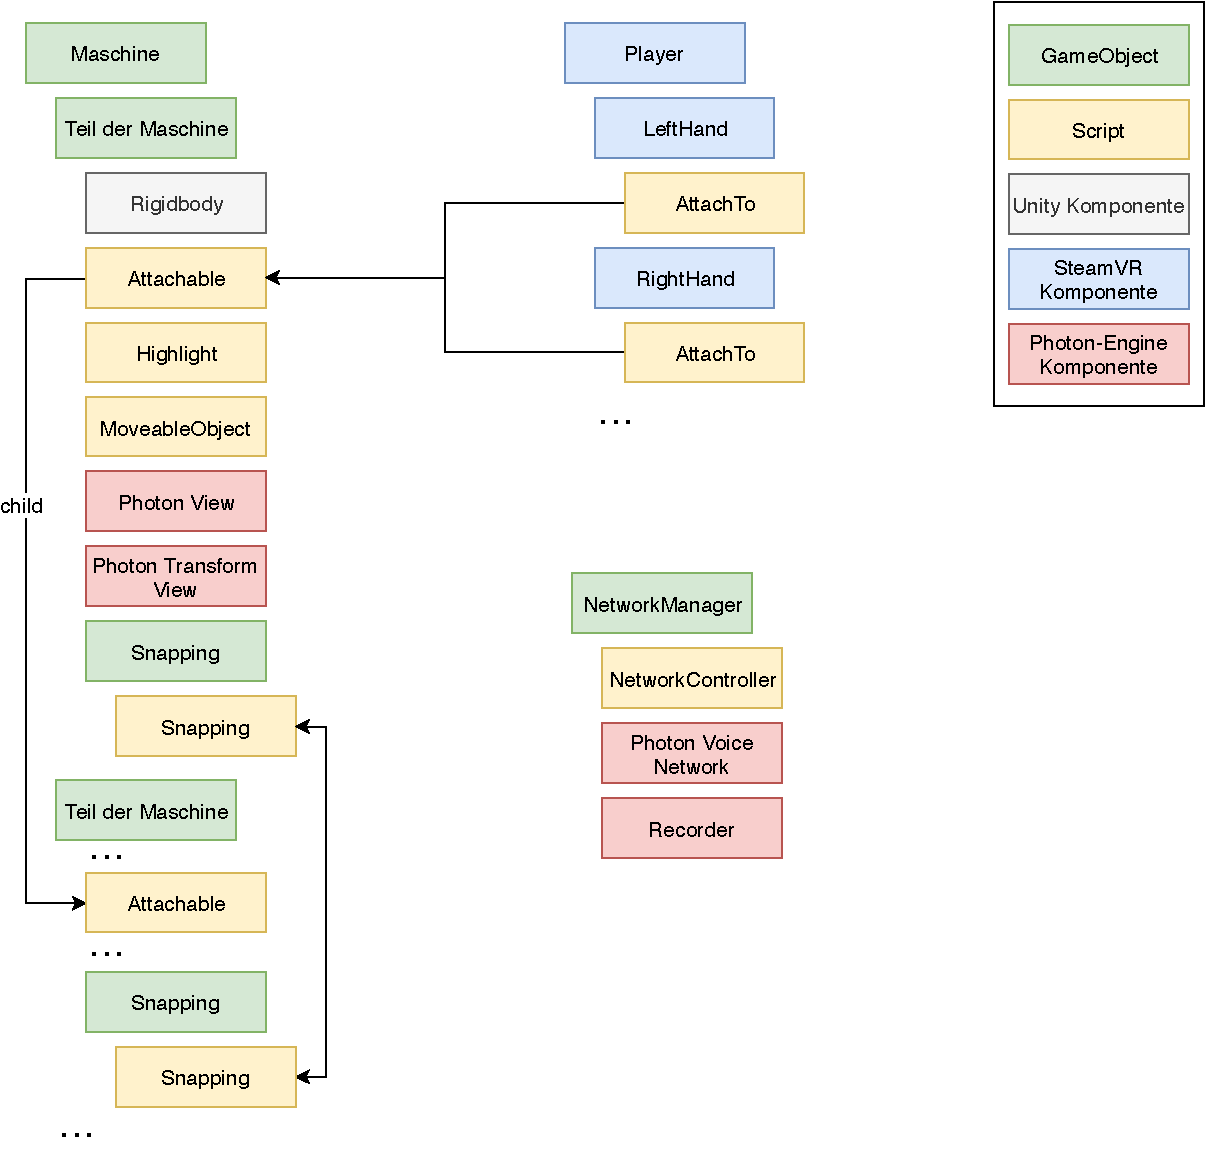
\includegraphics[keepaspectratio,width=0.65\linewidth]{img/Klassendiagramm_T2.pdf}
	\caption{Klassendiagramm des Multi-User Prototypen}
	\label{fig:klassendiagramm_multi_user}
\end{figure}

Viele Skripte und Komponenten sind die gleichen wie beim Single-User Prototypen, beschrieben in Kapitel \ref{ch:klassendiagram_single_user}. Dementsprechend werden hier nur die neuen oder geänderten Komponenten beschrieben. \\
Der \grqq NetworkController\grqq{} ist für die Verbindungsaufnahme zu der Photon-Engine verantwortlich. Die Komponenten \grqq Photon Voice Network\grqq{} und \grqq Recorder\grqq{} stammen aus dem Photon-Voice Plugin und sind für die Kommunikation zwischen den Benutzer zuständig, beschrieben in Kapitel \ref{ch:kommunikation_zwischen_benutzern_realisierung}. \\
Das Skript \grqq Attachable\grqq{} funktioniert ähnlich wie bisher. Einziger Unterschied ist der Ablauf beim greifen eines Objektes. Hier ruft das Skript erst noch die Funktion \textit{RequestOwnership()} auf um Besitzer des Objektes zu werden, beschrieben in Kapitel \ref{ch:gleichzeitige_interaktion_realisierung}. \\
Das Skript \grqq MovableObject\grqq{} zusammen mit den beiden Komponenten \grqq Photon View\grqq{} und \grqq Photon Transform View\grqq{} sind dafür zuständig, dass die Objekte zwischen den Instanzen synchronisiert werden, beschrieben in Kapitel \ref{ch:multi_user}.